\section{A Classification Framework for SoTS}\label{sec:literature-review-classification}

To organize how DT and SoS concepts are combined, we develop a classification framework grounded in classical SoS theory~\cite{maier1998architecting, maier2014role} and foundational DT concepts~\cite{kritzinger2018digital}. The framework is derived using a mixed sample-case generalization approach~\cite{jwieringa2015six}, where studies from the corpus (\secref{sec:literature-review-study-design}) are decomposed into architectural abstractions to identify recurring patterns.

\subsection{Core Elements}
The framework is based on a small set of core architectural elements. A \textit{System} is the fundamental building block of a SoS and may be composed hierarchically of other systems. In SoTS, systems may be associated with \textit{Physical Twins} and corresponding \textit{Digital Twins}. A key distinction is how components are coupled. SoS constituents typically interact through weak coupling, allowing for independent operation and decision-making. In contrast, DTs maintain strong coupling with their physical counterparts through continuous data exchange and feedback. Some architectures also introduce a coordinating element responsible for system-level decisions. This \textit{controller} may be implemented as a higher-level DT or supervisory component that aggregates information and coordinates behaviour across constituents. These elements form the basis for identifying recurring SoTS architectural patterns.

\subsection{Instances}
\begin{figure}[H]
\centering

% --- Row 1 ---------------------------------------------------
\subfloat[Directed SoTS]{%
    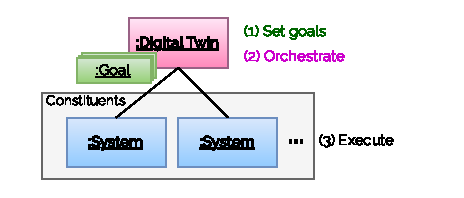
\includegraphics[trim={0.66cm 0.25cm 1.1cm 0.25cm},clip,
    width=0.4\linewidth]{figures/Literature Review/framework/instances/directed.pdf}}
\hfill
\subfloat[Acknowledged SoTS]{%
    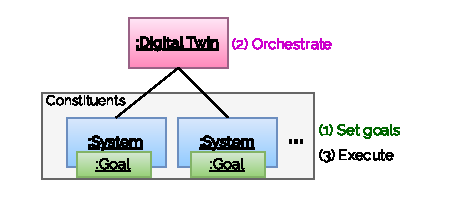
\includegraphics[trim={0.66cm 0.25cm 1.1cm 0.25cm},clip,
    width=0.4\linewidth]{figures/Literature Review/framework/instances/acknowledged.pdf}}
\\[1.2em]

% --- Row 2 ---------------------------------------------------
\subfloat[Collaborative SoTS]{%
    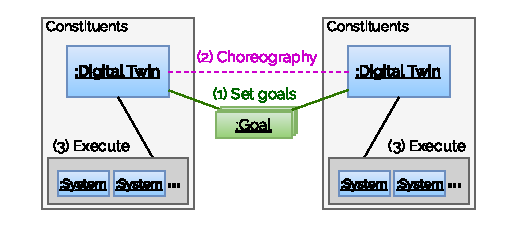
\includegraphics[trim={0.66cm 0.25cm 0.75cm 0.25cm},clip,
    width=0.4\linewidth]{figures/Literature Review/framework/instances/collaborative.pdf}}
\hfill
\subfloat[Virtual SoTS]{%
    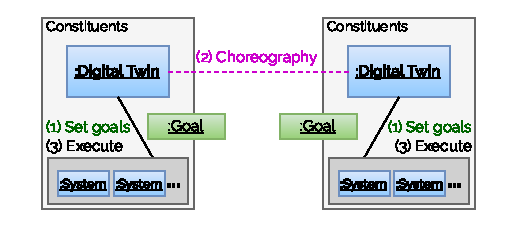
\includegraphics[trim={0.66cm 0.25cm 0.75cm 0.25cm},clip,
    width=0.4\linewidth]{figures/Literature Review/framework/instances/virtual.pdf}}
\\[1.2em]

% --- Row 3 ---------------------------------------------------
\subfloat[System of Specialized DTs]{%
    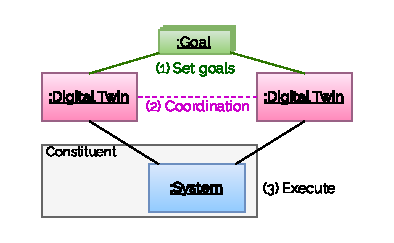
\includegraphics[trim={0.66cm 0.25cm 0.50cm 0.25cm},clip,
    width=0.4\linewidth]{figures/Literature Review/framework/instances/domainspec.pdf}}
\hfill
\subfloat[System of Specialized DTs and Specialized Systems]{%
    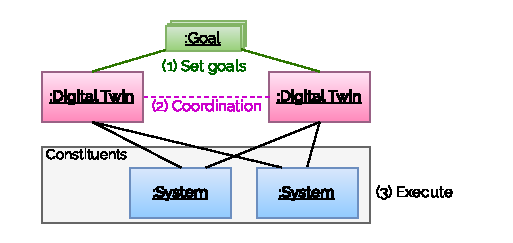
\includegraphics[trim={0.66cm 0.25cm 0.75cm 0.25cm},clip,
    width=0.4\linewidth]{figures/Literature Review/framework/instances/domainspec2.pdf}}

\caption{Overview of the six architectural styles observed in SoTS}
\label{fig:sots-architectures}
\end{figure}

Six recurring SoTS architectures are identified (\figref{fig:sots-architectures}). Four align with \citet{maier1998architecting}'s canonical SoS types---directed, acknowledged, collaborative, and virtual---while two reflect DT-specific specializations. Each architecture represents a different way of organizing control, coordination, and autonomy. \textbf{Directed SoTS} follow a hierarchical structure, where a central DT sets system-wide goals and coordinates other DTs. Constituents remain independent, but their behaviour is guided by the central controller. Goals are centrally defined and enforced. \textbf{Acknowledged SoTS} also include a central DT, but it coordinates rather than controls. Each DT maintains its own local goals, and system behaviour emerges through coordination. Goals are locally defined but aligned through the central DT. \textbf{Collaborative SoTS} remove the central controller. DTs coordinate directly with each other, working together through peer-to-peer interaction. Goals are shared and achieved through distributed coordination. \textbf{Virtual SoTS} go further, with fully autonomous DTs that define their own goals. They form and dissolve connections dynamically, and coordination emerges from local decisions. Goals are dynamic and may emerge at runtime.

Two additional architectures arise from DT specialization. These are not observed in the current corpus but are included as extensions of the framework and are expected to emerge in future systems. A \textbf{System of Specialized DTs} consists of multiple DTs representing different aspects of the same physical system. These DTs must coordinate to maintain consistent views and support joint decisions. Coordination is required to reconcile partial system representations. The \textbf{System of Specialized DTs and Systems} extends this across multiple systems, where specialized DTs coordinate across system boundaries using shared models or standards rather than a central controller. Coordination is achieved through shared semantics or interoperability mechanisms.